\chapter{Моделирование деградации РТГС на основе $Al_{x}Ga_{1−x}As$}
На основе выше исследованных параметров и полученных моделей получим модель деградации РГТС на основе $AlGaAs$.

В схема исследуемой на диффузионное расплытие модели приведена на рис.\ref{fig:RTHSModelDiff}

\begin{figure}
	\centering
	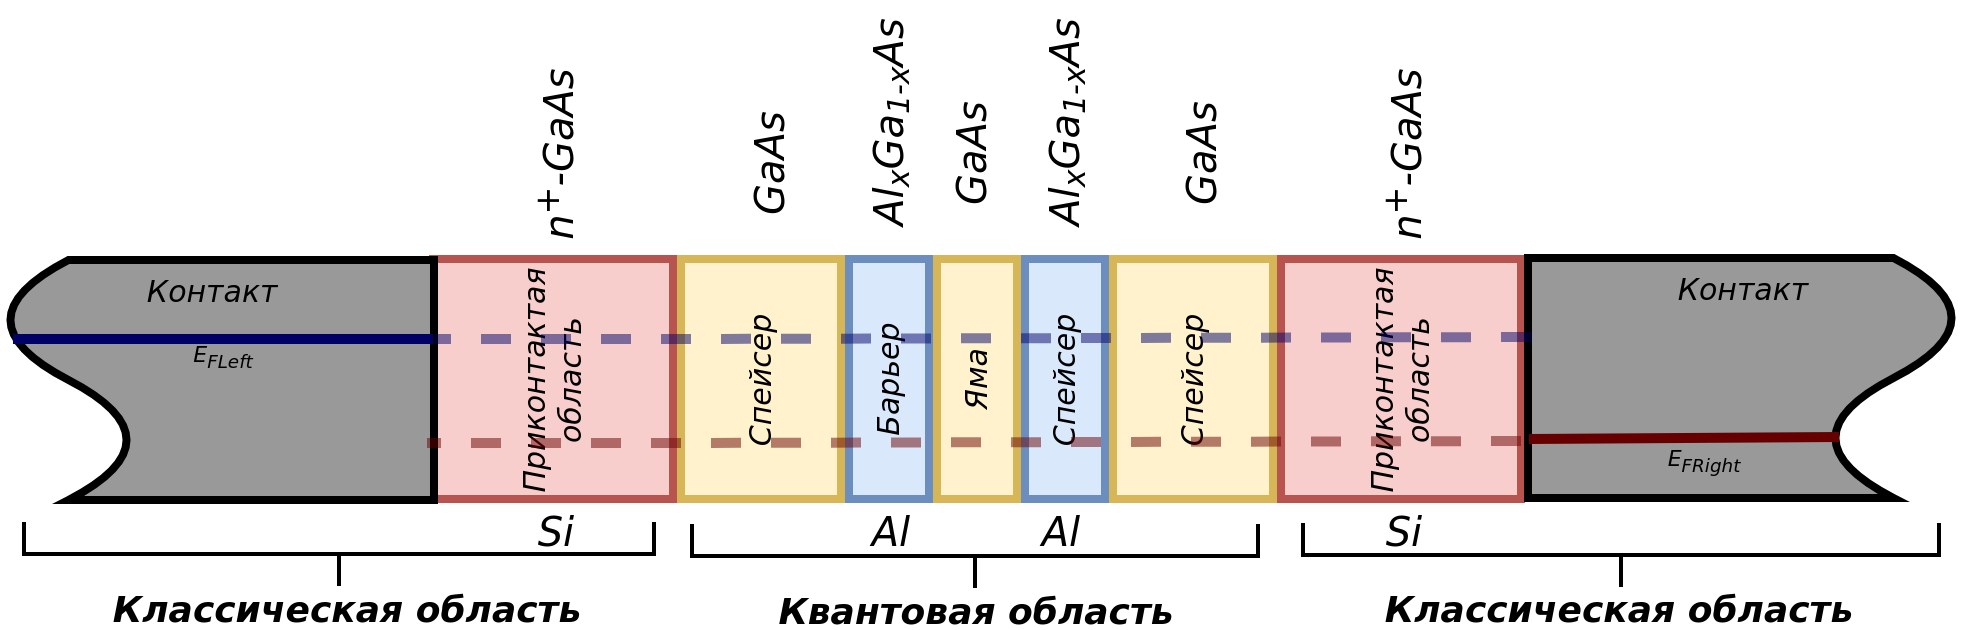
\includegraphics[width=0.9\linewidth]{assets/RTHSModelDiff}
	\caption{Стуктура РТГС для моделирования диффузии}
	\label{fig:RTHSModelDiff}
\end{figure}

В данной модели возможны:
\begin{itemize}
	\item Диффузия $Al$ из барьеров в яму;
	\item Диффузия $Si$ из приконтактных областей в активную область.
\end{itemize}

Рассмотрим диффузионное расплытие активной области и проникновение легирующий примеси отдельно.

Размеры нашей модели:
\begin{itemize}
	\item Спейсер: $a = 10$ монослоев;
	\item Барьер: $b = 6$ монослоев;
	\item Яма: $a = 6$ монослоев;
\end{itemize}

\begin{figure}
	\centering
	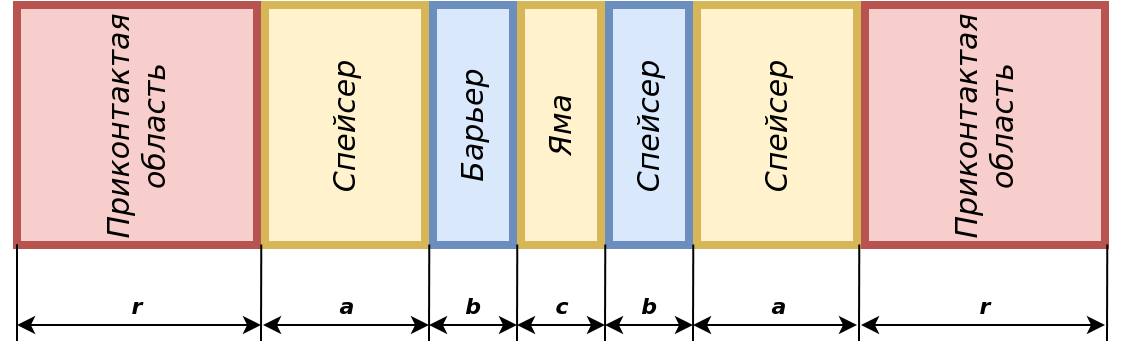
\includegraphics[width=0.7\linewidth]{assets/RTHS}
	\caption{Размеры РТГС}
	\label{fig:RTHS}
\end{figure}

\section{Диффузионное расплытие активной области}
Диффузионное расплытие активной области в случаи чистых полупроводников подчиняется (\ref{eq:DConst}). Коэффициент диффузии постоянен и скорость ухода части $Al$ с границ активной области равен скорости их прихода -- это соответствует конечно-разностной схеме (\ref{eq:DDiffConst}).

Температуру ГС ($T$) выберем равной $800\,K$. Время воздействия: $1$, $5$, $10$ лет.

\begin{figure}[h!]
	\centering
	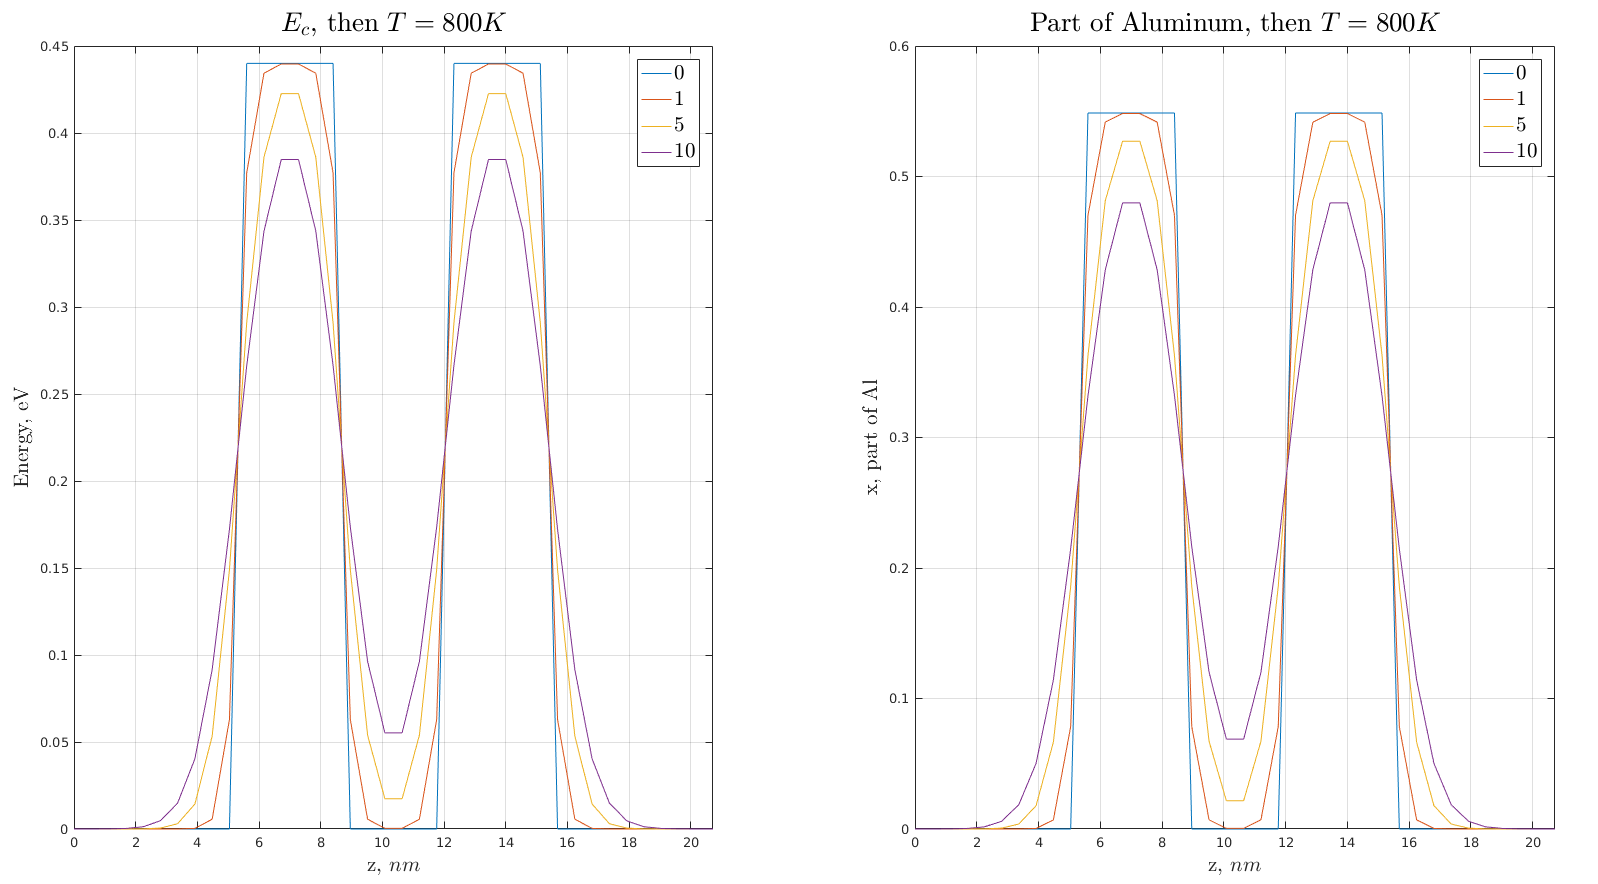
\includegraphics[width=0.93\linewidth]{DOAlGaAs}
	\caption{Расплытие потенциального рельефа чистого $Al_{x}Ga_{1−x}As$}
	\label{fig:DOAlGaAs}
\end{figure}

\begin{figure}[h!]
	\centering
	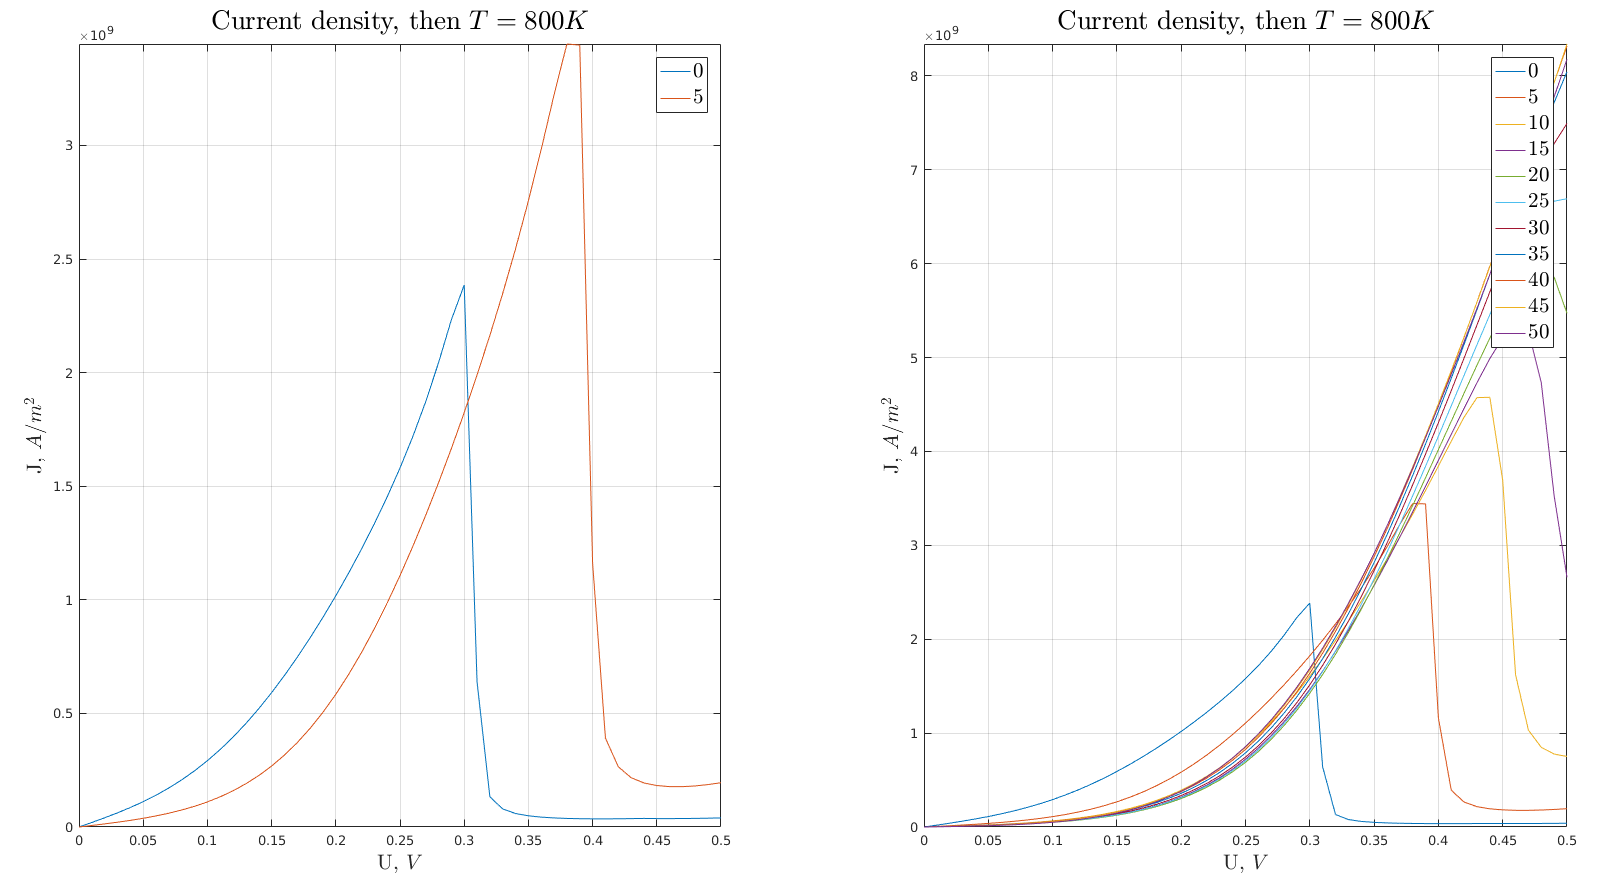
\includegraphics[width=0.94\linewidth]{JDOAlGaAs}
	\caption{Деградация тока через РГТС на основе чистого $Al_{x}Ga_{1−x}As$}
	\label{fig:JDOAlGaAs}
\end{figure}

В процессе деградации ГС уменьшается ширина и глубина ПЯ (рис.~\ref{fig:DOAlGaAs}).

Как видно из рис.~\ref{fig:JDOAlGaAs} в результате деградации увеличивается пиковое напряжение и величина пикового тока, что соответствует ранее полученным результатам.

Так как невозможно получить чистный полупроводник, в нем всегда присутствует донорная примесь, которая увеличивает скорость диффузии, что соответствует (\ref{eq:DNd}).

\begin{figure}[h!]
	\centering
	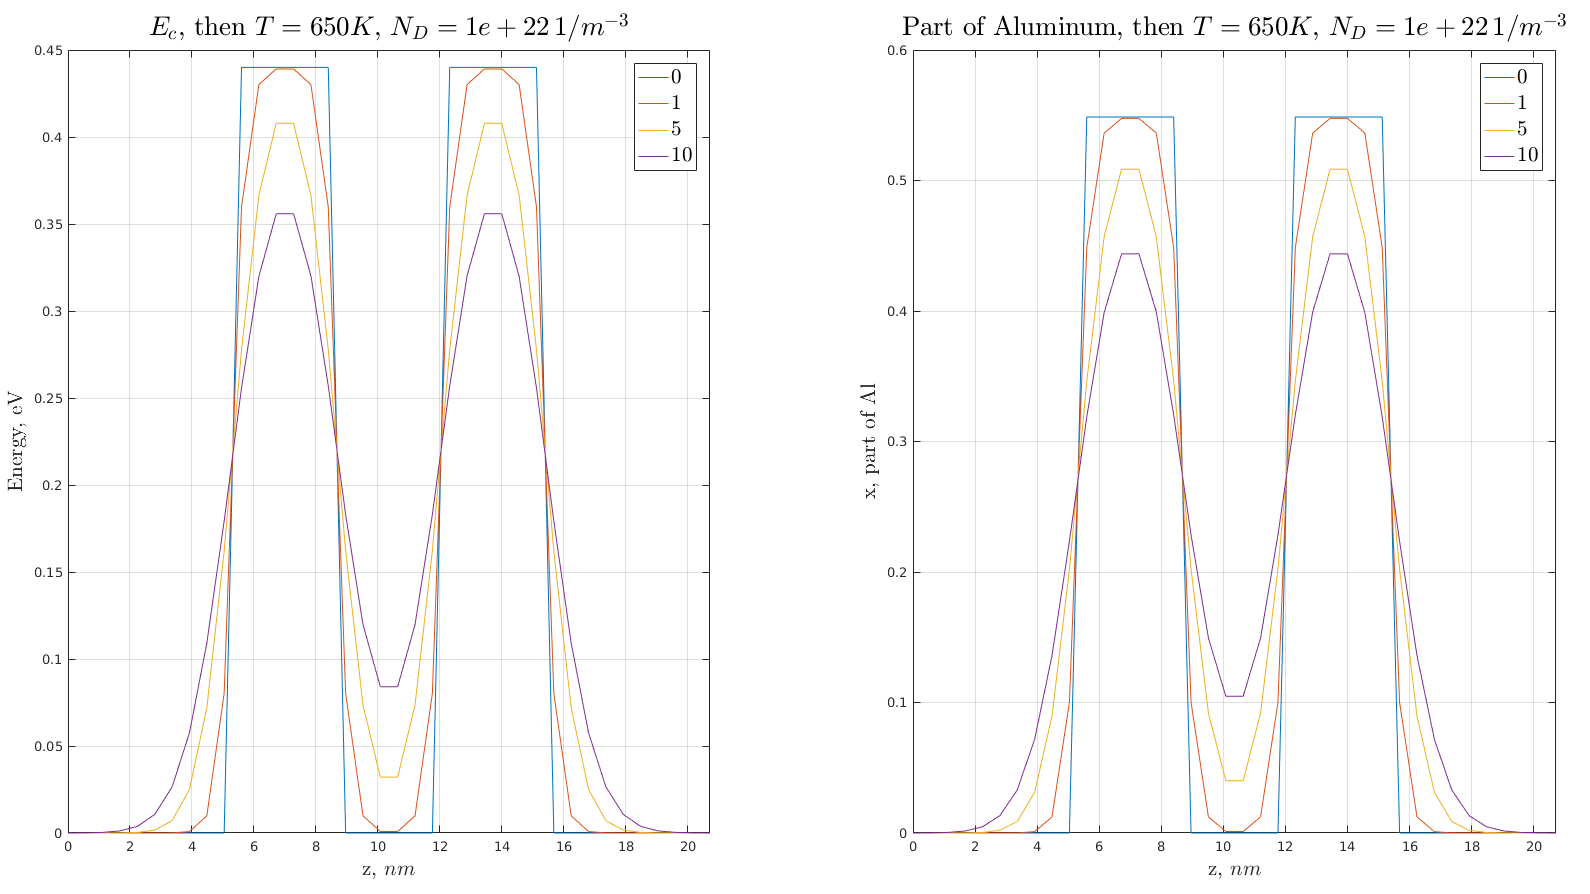
\includegraphics[width=0.8\linewidth]{DOAlGaAsNd}
	\caption{Расплытие потенциального рельефа $Al_{x}Ga_{1−x}As$ при наличии донорной примеси $N_{D}=10^{22}\, 1/m^{3}$} 
	\label{fig:DOAlGaAsNd}
\end{figure}

\begin{figure}[h!]
	\centering
	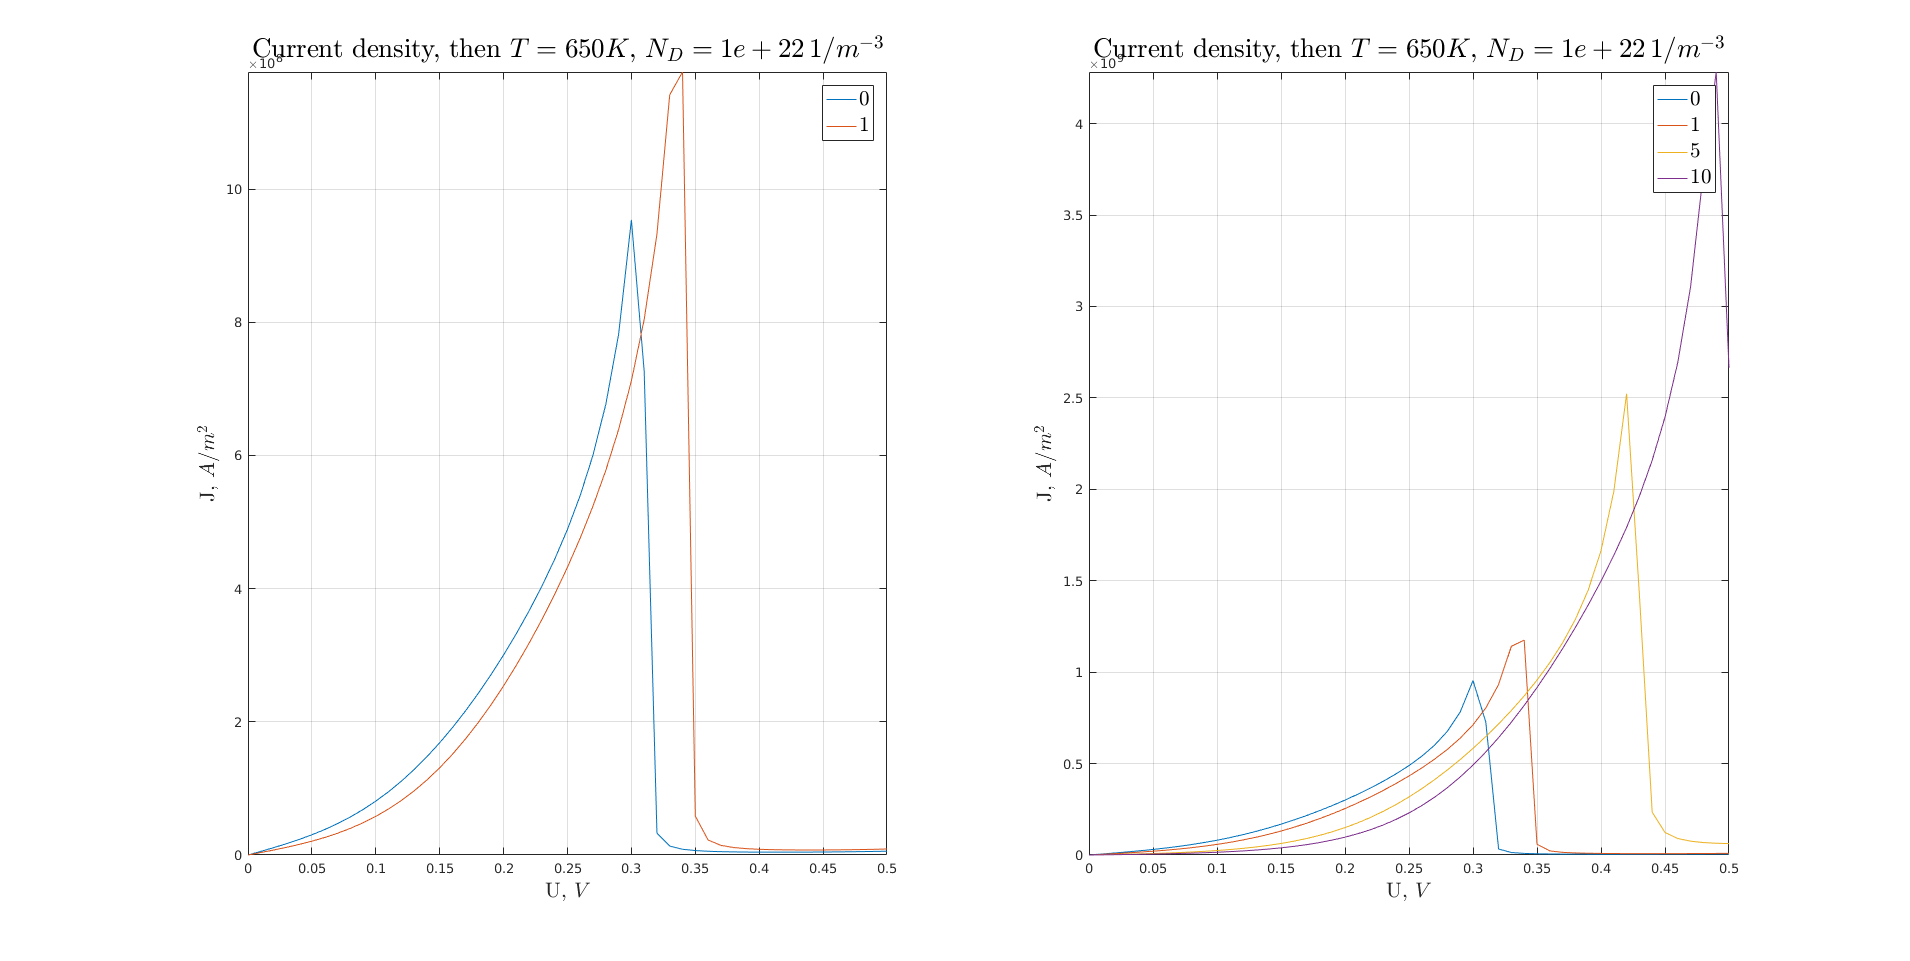
\includegraphics[width=0.8\linewidth]{JDOAlGaAsNd}
	\caption{Деградация тока через РГТС на основе $Al_{x}Ga_{1−x}As$ при наличии донорной примеси $N_{D}=10^{22}\, 1/m^{3}$}
	\label{fig:JDOAlGaAsNd}
\end{figure}


Аналогичный результат деградации (рис.~\ref{fig:DOAlGaAsNd}) был получен при меньшей температуре $T = 650K$ и концентрации донорной примеси ($N_{D}$) $10^{22}\, 1/m^{3}$.

\subsection{Вывод}
В процессе деградации преобладающими факторами деградации ВАХ РТГС являются: уменьшение глубины и ширины ПЯ, которые увеличивают пиковое напряжение и пиковый ток.

Наличие донорной примеси ускоряет процесс деградации ГС. При это из-за сильно экспоненциальной зависимости коэффициента диффузии скорость диффузии при комнатных температурах не существенна ($T = 300K$).